\section{Results and Discussions}

\begin{figure*}[!h]
\centering     %%% not \center
\subfigure[Resource utilization for sigmoid Activation function]{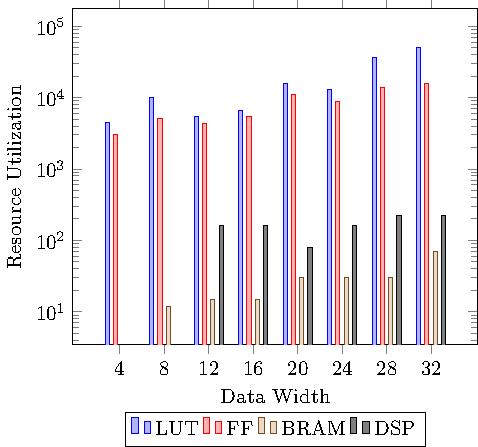
\includegraphics[width=0.65\columnwidth]{Figures/SigmoidResource.pdf}}
\subfigure[Resource utilization for ReLU Activation function]{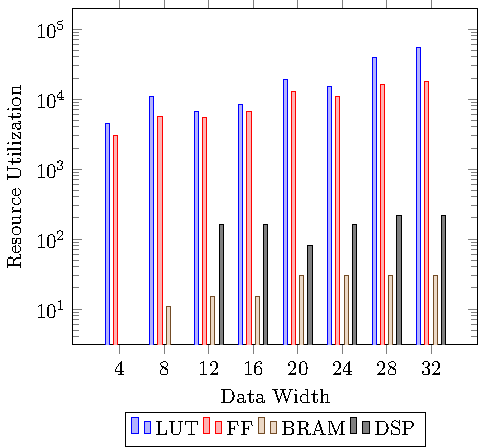
\includegraphics[width=0.65\columnwidth]{Figures/ReLUResource.pdf}}
\subfigure[Resource utilization for sigmoid Activation function with varying depth and datawidth 16]{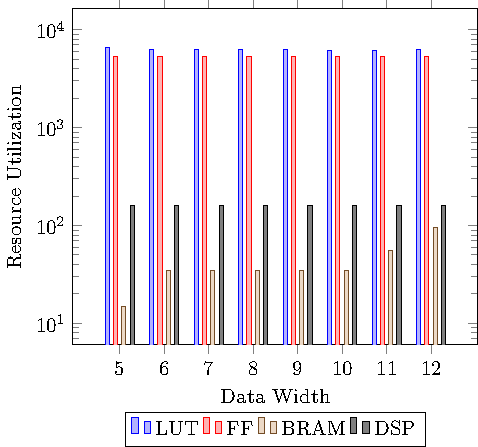
\includegraphics[width=0.65\columnwidth]{Figures/VarSigmoid16Width.pdf}}
\subfigure[Comparison of accuracy for Sigmoid and ReLU activation functions]
{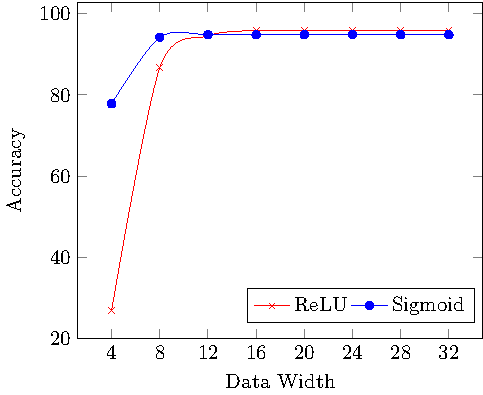
\includegraphics[width=0.62\columnwidth]{Figures/Accuracy.pdf}}
\subfigure[Detection accuracy and varying sigmoid memory depth]{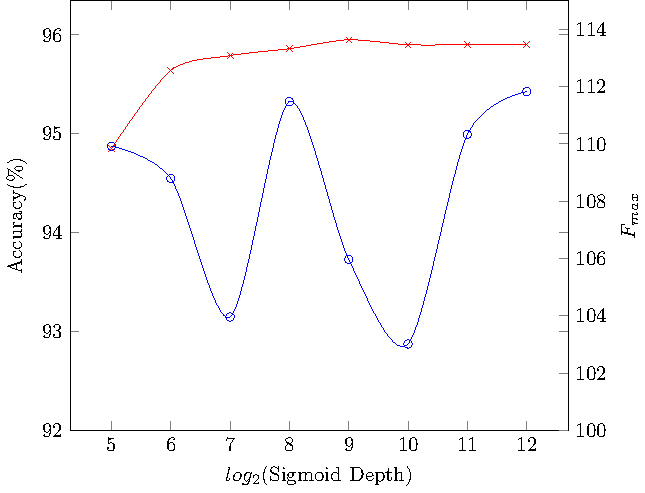
\includegraphics[width=0.65\columnwidth]{Figures/AccuracyVarSigmoid.pdf}}
\subfigure[Datawidth vs Maximum Frequency and Power consumption]{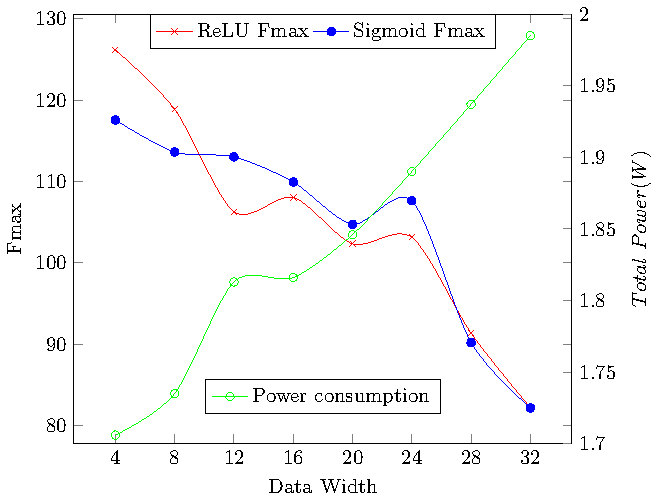
\includegraphics[width=0.65\columnwidth]{Figures/Timing.pdf}}
\caption{Evaluation results in terms of resource utilization, power consumption and maximum clock performance for different neural networks generated by ZyNet}
\end{figure*}

In this section we discuss the implementation results and performance of ZyNET based DNNs.
Multiple DNNs targeting the popular MNIST dataset is implemented and evaluated through both simulation and hardware validation.
The popular dataset for handwritten digit recognition uses 30000 images for training and 10000 images for testing.
The weights and biases for the network was initially determined through the corresponding software implementation and used for pre-training hardware implementation.
The software implementation with 30 epoch training provides 96.52\% detection accuracy for the testing set.

All implementations follow a 5 layer architecture with 784 neurons in input layer, 2 hidden layers with 30 neurons each and 1 hidden layer with 10 neurons and an output layer with 10 neurons.
The output layer is connected to a \emph{hardmax} module to detect the neuron with maximum output value.
All designs are simulated and implemented with Xilinx Vivado 2018.3 version and hardware validated on ZedBoard having an XC7Z020-CLG484 SoC and 512MB external DDR3 memory. 
All implementations use Vivado default settings and do not apply any optimization (timing,area or power). 

The DNN implementation was evaluated for both Sigmoid and ReLU activation functions for varying datawidth.
Fig.~\ref{fig:accuracy} shows the relation between the detection accuracy and datawidth.
It could be seen that for very small datawidth (such as 4 and 8 bits), Sigmoid-based function implementation outperforms ReLU-based implementation.
As the width increases, ReLU has slight advantage over Sigmoid implementation and accuracy of both implementations becomes constant beyond 12-bits.
Sigmoid implementation gives a maximum of 94.86\% detection accuracy and ReLU gives a maximum of 95.87\%.
The degradation in the result compared to software implementation can be attributed to the error introduced due to fixed point representation of weights, biases and input data.
Still the approximation causes less than 1\% error but gives considerable advantage in terms of resource utilization and clock performance.

Figures~5(a) and 5(b) compares the resource utilization of the DNNs for different data widths in terms of LUTs, flip-flops, Block RAMs and DSP slices while using the two different activation functions.
Since the RTL code generated by ZyNet does not explicitly instantiates any IP cores, for smaller designs the implementation tool (Vivado) automatically maps the multipliers and weight memory blocks into LUTs and flip-flops.
For larger data size, the lookup table used for implementing Sigmoid function are mapped to Block RAMs, which considerably increases the BRAM utilization.
For example, for 32-bit implementation, Sigmoid-based implementation requires 50350 LUTs, 15544 flip-flops, 70 BRAMs and 220 DSP slices.
At the same time ReLU-based implementation requires 54559 LUTs, 18074 flip-flops, 30 BRAMs and 220 DSP slices.
These numbers roughly maps to 94.6\% LUTs, 17\% flip-flops, 21.4\% BRAMs and 100\% DSP slices of xc7z020clg484-1 chip used in the Zed Board.
It should be noted that 16-bit implementation also consumes 220 DSP slices and as discussed before for larger networks the tool automatically maps the multipliers into LUTs and flip-flops.
Thus the largest network size is constrained by the number of LUTs available in the device. 

Another interesting result is the size of the Sigmoid look-up-table and the detection accuracy.
Fig.~5(e) shows the relation between the number of address bits used for Sigmoid LUT (sigmoid memory depth is $2^{address \_bits}$) and detection accuracy.
Here the datawidth is kept at a constant value of 16.
Experiments showed that the accuracy is quite low when the number of address bits is less than the sum of integer bits used to represent input values and weight values.
Here the minimum value is set as 5 bits, since the implementation uses 1-bit integer value for input and 4-bits for weight.
It could be seen that the Accuracy initially increases and remains constant after 8 bits.
Comparing it with Fig.~5(c), it could be seen that the resource utilization remain constant between LUT address width 6 to 10.
At the same time detection accuracy increases from 95.64\% to 95.95\% between these values.
The constant resource utilization is attributed the granularity of BRAM available in the device, which is 18Kb for 7-series Xilinx FPGAs.
Beyond 10-bits, resource utilization increases due to more BRAMs are required for implementing Sigmoid LUTs.
The detection accuracy also slightly reduces (95.90\%) remains constant.
The maximum clock frequency varies between 103~MHz and 111~MHz due to placement algorithm of the implementation tool.

Fig.~4(f) shows the maximum clock performance of the DNN for varying datawidth with two activation functions.
In most cases Sigmoid implementation outperforms ReLU implementation, but on Zynq platforms most of the other design components will be running at 100MHz, which is achieved by both implementations upto 24-bit wide implementations.
The plot also shows the power consumption of ZedBoard for Sigmoid-based network when running at 100 MHz clock frequency.
It varies between 1.706~W and 1.985~W depending on the datawidth (resource utilization).
Comparing it with the other popular edge device Raspberry-Pi3, the power consumption is in the range of 2.7W to 3.1W. 

Finally comparing the throughput, ZyNet based network on ZedBoard running at 100 MHz has a detection speed of 7.84 us/sample. On a Raspberry Pi3 platform using tensor flow, the throughput is 266 us/sample. On a standard computer with Intel i7 processor and 16GB RAM, the throughput for the same network is 30us/sample. This clearly demonstrates the advantage of reconfigurable platforms for edge devices in terms of throughput and power consumption.